\section{Auto MPG dataset}
\label{db:sec:ds1}
\subsection{Description}
Auto MPG contains 8 attributes of 398 cars  and their corresponding MPG (Miles Per Gallon) value. The dataset has some missing value in its forth column (horsepower). Shortage of data as well as the existence of some missing values makes the dataset distinct and interesting for ML. Furthermore because of its short execution time, it provided us the opportunity to apply all developed algorithms as well as imputation techniques.

\subsection{Preprocessing}
In order to standardize data, we used standard scale which first transforms the data to center it by removing the mean value of each feature and then scales it by dividing non-constant features by their standard deviation \cite{scikitstandardization}.

In order to impute missing values, we applied three different techniques containing calculating Mean, Median and Most-Frequent value.

\subsection{Regression}
\subsubsection{Linear Regression}
The results of different Linear Regression algorithms with different imputation techniques are shown in Table~\ref{table:db1-linearregression}. Ridge Regression was tested by different values for $\alpha$ ($0.1$, $0.5$, $1$ and $10$) and $0.1$ seems to be the best value. The final results were very similar. It showed all the values are rather the same and very biased. By reducing the number of instances in Train Data the final bias reduced significantly. In order to improve the results, we used Multinomial Regression in the next step.

\subsubsection{Polynomial Ridge Regression}
By adding more attributes to the linear algorithm, we could apply the data on Polynomial Ridge Regression. Regarding to very short execution time, we tried many different exponent values and achieved novel results. As it is shown in Table~\ref{table:db1-polynomialregression}, till exponent value five there is no big difference between linear and polynomial model. In contrast to the exponent values around ten, value ten creates a surprisingly good model. It happens again in some other numbers like $22$ and we achieved a very good result in $32$. One interesting point is that when the results are very biased (like fifteen), the higher we chose $\alpha$, the better were our results.

\subsection{$k$-nearest neighbor}
In the first three runs, $1, 5$ and $10$ were selected as the number of neighbors ($k$). Since by increasing $k$, the final result seemed to be better, we continued increasing the value and found $18$ as a reasonable value. The results for different imputation techniques are depicted in Table~\ref{table:db1-nearestneighbor}. In this case, mean value for imputation seems better than other techniques.

\subsection{Support Vector Machine}
We applied the SVM algorithm with default parameters presented by sci-kit. The default mode of the algorithm uses $\epsilon$ equal to $0.1$, $\gamma$ equal to $0$ and RBF as kernel. The results for three different imputation techniques is shown in Table~\ref{table:db1-SVM}. Changing the imputation technique doesn't seem to have any considerable effect on the results.

\subsection{Stochastic Gradient Descent}
We used Huber and Squared Loss as loss functions for the SGD algorithm. Four $\epsilon$ values from the range of $100$ to $2000$ were selected for Huber loss function. The results applied for three different imputation techniques is shown in Table~\ref{table:db1-SGD}. In the final result, Squared Loss seemed to be the best Loss Function and Mean the best imputation technique.

\subsection{Neural Networks}
As the last part, we also apply neural networks model on the dataset. We picked Mean value as imputation technique and as it is shown in Table~\ref{table:db1-NeuralNetwork}, different hidden layers and node counts were applied. Based on achieved results, regardless to number of layers, having ten to twenty nodes usually leads to the best results. Using one hidden layer seems to be the best model. In current data one layer and twenty nodes seems to be the best model. It should also be considered that different runs return different results while not very diverse.

\subsection{Comparison}
Table~\ref{table:db1-results} shows the comparison between the best results of each algorithm.

Based on the results the following conclusions can be obtained:
\begin{itemize}
  \item Polynomial Ridge Regression has the best results and SVM creates the second best one.
  \item While good results in Polynomial Ridge Regression, standard deviation of bias between results and real values is rather high. Between all algorithms, SVM seems more stable.
  \item Regarding to amount of data, SGD is an inappropriate model.
  \item Although all the algorithms are executing less than one second, Neural Networks has the longest execution time and SGD the shortest.
  \item Mean is the best Imputation technique among the implemented ones.
\end{itemize}

		\begin{table}
\begin{center}
\begin{tabular}{|p{4cm}|c|c|c|c|}
\hline Algorithm and Parameters & Imputation & Bias Mean & Bias Std & Execution Time(s)\\

\hline Linear Ridge Regression, $\alpha=0.1$ & Mean & $9.152$ & $3.891$ & $00.027$ \\

\hline Polynomial Ridge Regression, highest exponent$=32$, $\alpha=0.1$ & Mean & $\mathbf{1.127}$ & $2.895$ & $00.155$  \\

\hline nearest neighbors $k=18$ & Mean & $6.62$ & $3.36$ & $00.02$  \\

\hline SVM & Mean & $5.76$ & $\mathbf{2.044}$ & $00.118$  \\

\hline SGD, loss function$=$squaredloss & Mean & $8.682$ & $3.87$ & $\mathbf{00.003}$  \\

\hline Neural Networks, Hidden Layers$=1$, Nodes Count$=20$ & Mean & $6.25$ & $3.47$ & $00.83$  \\

\hline
\end{tabular}
    \caption{Auto MPG - Comparison between best results}
    \label{table:db1-results}
\end{center}
    \end{table}


\begin{figure}
	\center
	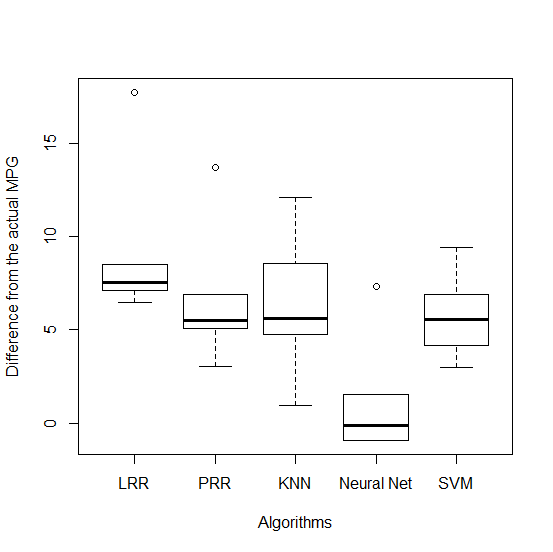
\includegraphics[scale=\figurescaling]{figures/mpg_bestresults.png}
	\caption{Auto MPG - Comparison between best results\label{fig:db1-mpg_bestresults}}
\end{figure}
